\section{Introduction}

The EHDA setup used in the lab for this project can be seen in the Figure 2.
For this project we are going to focus on nozzle to plate configuration and the high voltage
will be applied to the nozzle.
We use a variety of liquids to make the experiment such as ethyleneglycol + HNO3, ethanol, water + ethanol and 2-propanol.
Those liquid properties were already been analysed and considered in the automation routine.
The experiment can be made by voltage steps or voltage ramp. Both of the dynamics are being tested.
The flowrate is still being used as a constant.

\begin{figure}[H]
    \center
    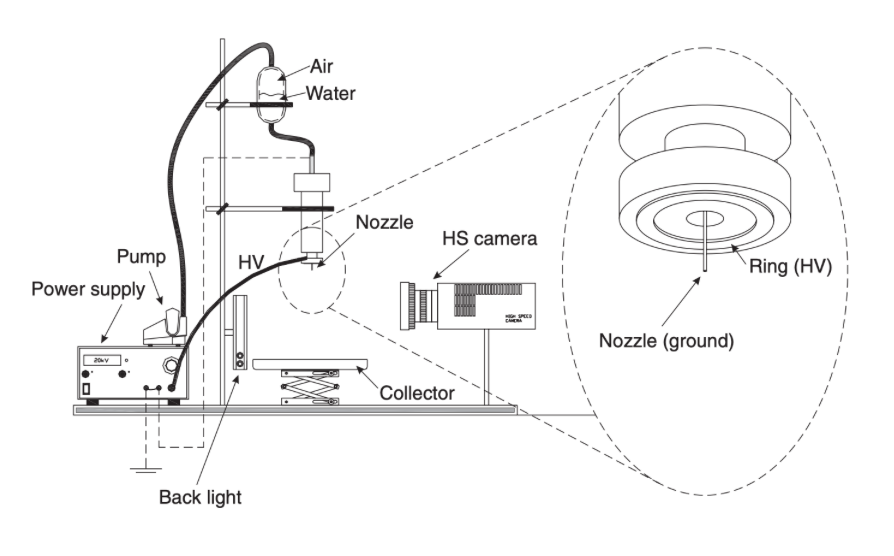
\includegraphics[width=8cm]{images/system_setup.png}
    \label{img3}
    \caption{system setup}
\end{figure}